\documentclass[10pt]{article}

\usepackage[T1]{fontenc}
\usepackage[utf8]{inputenc}
\usepackage[english]{babel}
\usepackage[margin=0.8in]{geometry}
\usepackage{setspace}
\usepackage{amsmath}
\usepackage{booktabs}
\usepackage{graphicx}
\usepackage{array}
\usepackage{tabularx}
\usepackage{microtype}
\usepackage[hidelinks]{hyperref}

\setstretch{1.03}
\setlength{\parindent}{0pt}
\setlength{\parskip}{0.45em}
\setlength{\textfloatsep}{10pt}
\renewcommand{\arraystretch}{1.12}

\begin{document}

\begin{center}
    {\Large \textbf{GFlowNets and Active Learning for Budgeted Scrabble Exploration}}\\
    \vspace{0.35em}
    \textbf{Final Project Report}\\
    \textbf{IFT 3710 / IFT 6759 --- Winter 2026}
\end{center}

\textbf{Team:} Yohan Zytoon, Charbel Gebrael, Yann-Olivier Jean

\section{Abstract}
This project studies budgeted discovery in a discrete combinatorial environment: generate Scrabble words of length at most \(7\), query an expensive oracle for their exact score, and discover strong valid words using as few real oracle calls as possible. The repository implements five main components: random dataset generation, a supervised baseline, a standard active-learning loop, a direct oracle-access GFlowNet, and a hybrid method that trains a GFlowNet on a cheap surrogate reward and uses active-learning style acquisition to decide which candidates deserve real oracle evaluation.

The main conclusion is consistent across the runs saved in the repository. A \emph{direct} GFlowNet is weak under a strict real-oracle budget because the reward is sparse and most random sequences are invalid. The hybrid method is more useful than the direct GFlowNet, but not because it should replace active learning entirely. Instead, it works best when the GFlowNet is used as a structured \emph{proposal generator} inside a larger loop that still relies on surrogate uncertainty, diversity-aware selection, and strict accounting of real-oracle cost. This is also the answer to the question ``why not just use a full GFlowNet in the hybrid model'': the expensive part of the problem is not generating candidates, but deciding which candidates are worth spending the limited real queries on.

\section{Problem Setting}
\subsection{Goal}
The project targets \emph{budgeted black-box optimization} over discrete strings. Each state is a padded sequence of up to \(7\) letters. The real oracle returns the exact Scrabble score if the sequence is a valid dictionary word and \(0\) otherwise. Under the main comparison protocol, each budget-matched method receives exactly \(1000\) real oracle queries.

\subsection{Why the problem is hard}
The search space is extremely large: even restricting attention to words of length \(3\) to \(7\), the number of raw sequences is
\[
\sum_{\ell=3}^{7} 26^\ell \approx 8.35 \times 10^9.
\]
Most of these sequences are not valid words, so the reward is highly sparse. In practice, this means that naive exploration produces a long stream of zeros, which is bad for both supervised surrogates and direct reward-driven generative models. The real challenge is therefore not only to maximize reward, but to do so \emph{sample-efficiently} under severe reward sparsity.

\subsection{Project objective}
The project was not only about finding a single best word. We also wanted to discover a \emph{good frontier} of candidates under budget. This is why the evaluation tracks both single-hit quality and frontier quality:
\begin{itemize}
    \item best score found,
    \item running top-10 mean,
    \item mean score over queried samples,
    \item valid-word ratio,
    \item query-efficiency metrics such as \(Q90\), the number of queries needed to reach \(90\%\) of a method's own final best score.
\end{itemize}

\section{What Was Implemented}
\subsection{Environment and infrastructure}
The environment extends the official Scrabble environment from the upstream \texttt{alexhernandezgarcia/gflownet} repository. This project adds:
\begin{itemize}
    \item a budget-aware oracle proxy,
    \item a surrogate-backed proxy that exposes fake rewards to the GFlowNet,
    \item experiment runners for dataset generation, baselines, active learning, direct GFlowNet, hybrid search, multi-seed comparisons, and ablations,
    \item result aggregation, paired significance tests, and report-ready visualizations.
\end{itemize}

\subsection{Dataset generation}
The repository supports several proposal distributions for random dataset creation and candidate generation:
\begin{itemize}
    \item uniform random letters,
    \item English letter-frequency sampling,
    \item score-biased letter sampling,
    \item vocabulary-derived bigram (\emph{n}-gram) sampling,
    \item bigram sampling further biased toward high-value Scrabble letters.
\end{itemize}
This matters because proposal quality is already a large part of the problem. The codebase gradually moved away from structure-agnostic sampling and toward vocabulary-aware generation because random strings are overwhelmingly invalid.

\subsection{Supervised baseline}
The supervised baseline trains a simple MLP with two heads:
\begin{itemize}
    \item a validity head that predicts whether a candidate is likely to be a real word,
    \item a score head that predicts score conditional on validity.
\end{itemize}
After training on a randomly labeled dataset, the model ranks a large candidate pool and spends the remaining real oracle budget on the top predicted candidates.

\subsection{Active learning}
The active-learning loop starts from a small seed set, then repeatedly:
\begin{enumerate}
    \item fits a surrogate model,
    \item samples a large candidate pool,
    \item scores candidates with an acquisition rule,
    \item selects a batch for real oracle evaluation,
    \item updates the labeled set.
\end{enumerate}
Two surrogate families are implemented:
\begin{itemize}
    \item Gaussian processes,
    \item deep ensembles.
\end{itemize}
Both surrogates use richer features than raw one-hot letters alone. In addition to one-hot sequence encodings, they use domain-inspired features such as word length, raw tile-score sum, vowel ratio, bigram plausibility, consonant-run statistics, and whether a sequence contains vowels at all.

The acquisition layer supports UCB, expected improvement, Thompson sampling, and uncertainty sampling. Batch selection is diversity-aware: instead of picking only the top-\(k\) by score, the code adds a Hamming-distance based diversity bonus to avoid wasting budget on near-duplicate strings.

\subsection{Direct oracle-access GFlowNet}
The direct GFlowNet uses the upstream implementation with trajectory-balance style training and MLP forward/backward policies. It receives \emph{real oracle reward} directly through the oracle proxy. This is the cleanest test of whether a standard GFlowNet can solve the problem without a surrogate.

\subsection{Hybrid method}
The hybrid method is the central contribution of the project. Its real logic is:
\begin{enumerate}
    \item collect an initial real labeled set,
    \item fit a surrogate on the real labels,
    \item once enough positive examples exist, train a GFlowNet on the surrogate reward instead of the real oracle,
    \item sample candidates from the GFlowNet,
    \item mix those candidates with random \emph{n}-gram samples, mutations of strong states, and local-search proposals,
    \item use an acquisition function to decide which mixed candidates receive real oracle queries,
    \item update the surrogate and occasionally refresh the GFlowNet.
\end{enumerate}

Several design choices in the final hybrid are important:
\begin{itemize}
    \item \textbf{Delayed activation:} the GFlowNet is not turned on immediately. In the comparison config, it starts only after round \(5\) and after at least \(20\) positive examples exist.
    \item \textbf{Warm starts:} when the surrogate-backed GFlowNet is retrained, it is warm-started from the previous one instead of being rebuilt from scratch conceptually.
    \item \textbf{Mixed proposal pool:} GFlowNet samples never fully replace random, mutation, or local-search candidates.
    \item \textbf{Plausibility bonus:} both acquisition and surrogate-backed GFlowNet rewards include a bigram-based plausibility bonus that nudges search toward word-like strings.
    \item \textbf{Separate cost accounting:} the code tracks real oracle queries, fake-oracle queries, and total cheap-model queries separately.
\end{itemize}

\subsection{Oracle-rich upper bound}
The repository also keeps a non-budget-matched GFlowNet upper bound. It is useful only as a ceiling: it answers ``what happens if real oracle access is much less constrained?'' It is \emph{not} a fair baseline, because it consumes around \(96{,}000\) real oracle calls in the archived \(5\)-seed comparison.

\section{Evaluation Protocol}
The most informative archived runs are:
\begin{itemize}
    \item \textbf{Tuned budget-matched sweep:} \texttt{2026-03-29\_21-12-32}, used by the report figures. This includes active learning, direct GFlowNet, and hybrid on \(5\) seeds, plus a baseline reference imported from \texttt{2026-03-29\_14-51-09}.
    \item \textbf{Complete five-method run:} \texttt{2026-03-29\_21-59-01}, which reruns baseline, active learning, direct GFlowNet, hybrid, and the oracle-rich upper bound together on \(5\) seeds.
\end{itemize}

All main comparisons use:
\begin{itemize}
    \item maximum word length \(7\),
    \item vocabulary checking enabled,
    \item \(1000\) real oracle queries for budget-matched methods,
    \item CPU execution.
\end{itemize}

\section{Results}
\subsection{Tuned budget-matched comparison}
Figure~\ref{fig:quality} and Figure~\ref{fig:dynamics} summarize the tuned \(5\)-seed budget-matched comparison used for the current report visualizations. The baseline shown in the table below is a reference baseline from the earlier run \texttt{2026-03-29\_14-51-09}; it was not rerun in the latest tuned sweep, so it should be read as contextual reference rather than part of a perfectly matched rerun.

\begin{figure}[t]
\centering
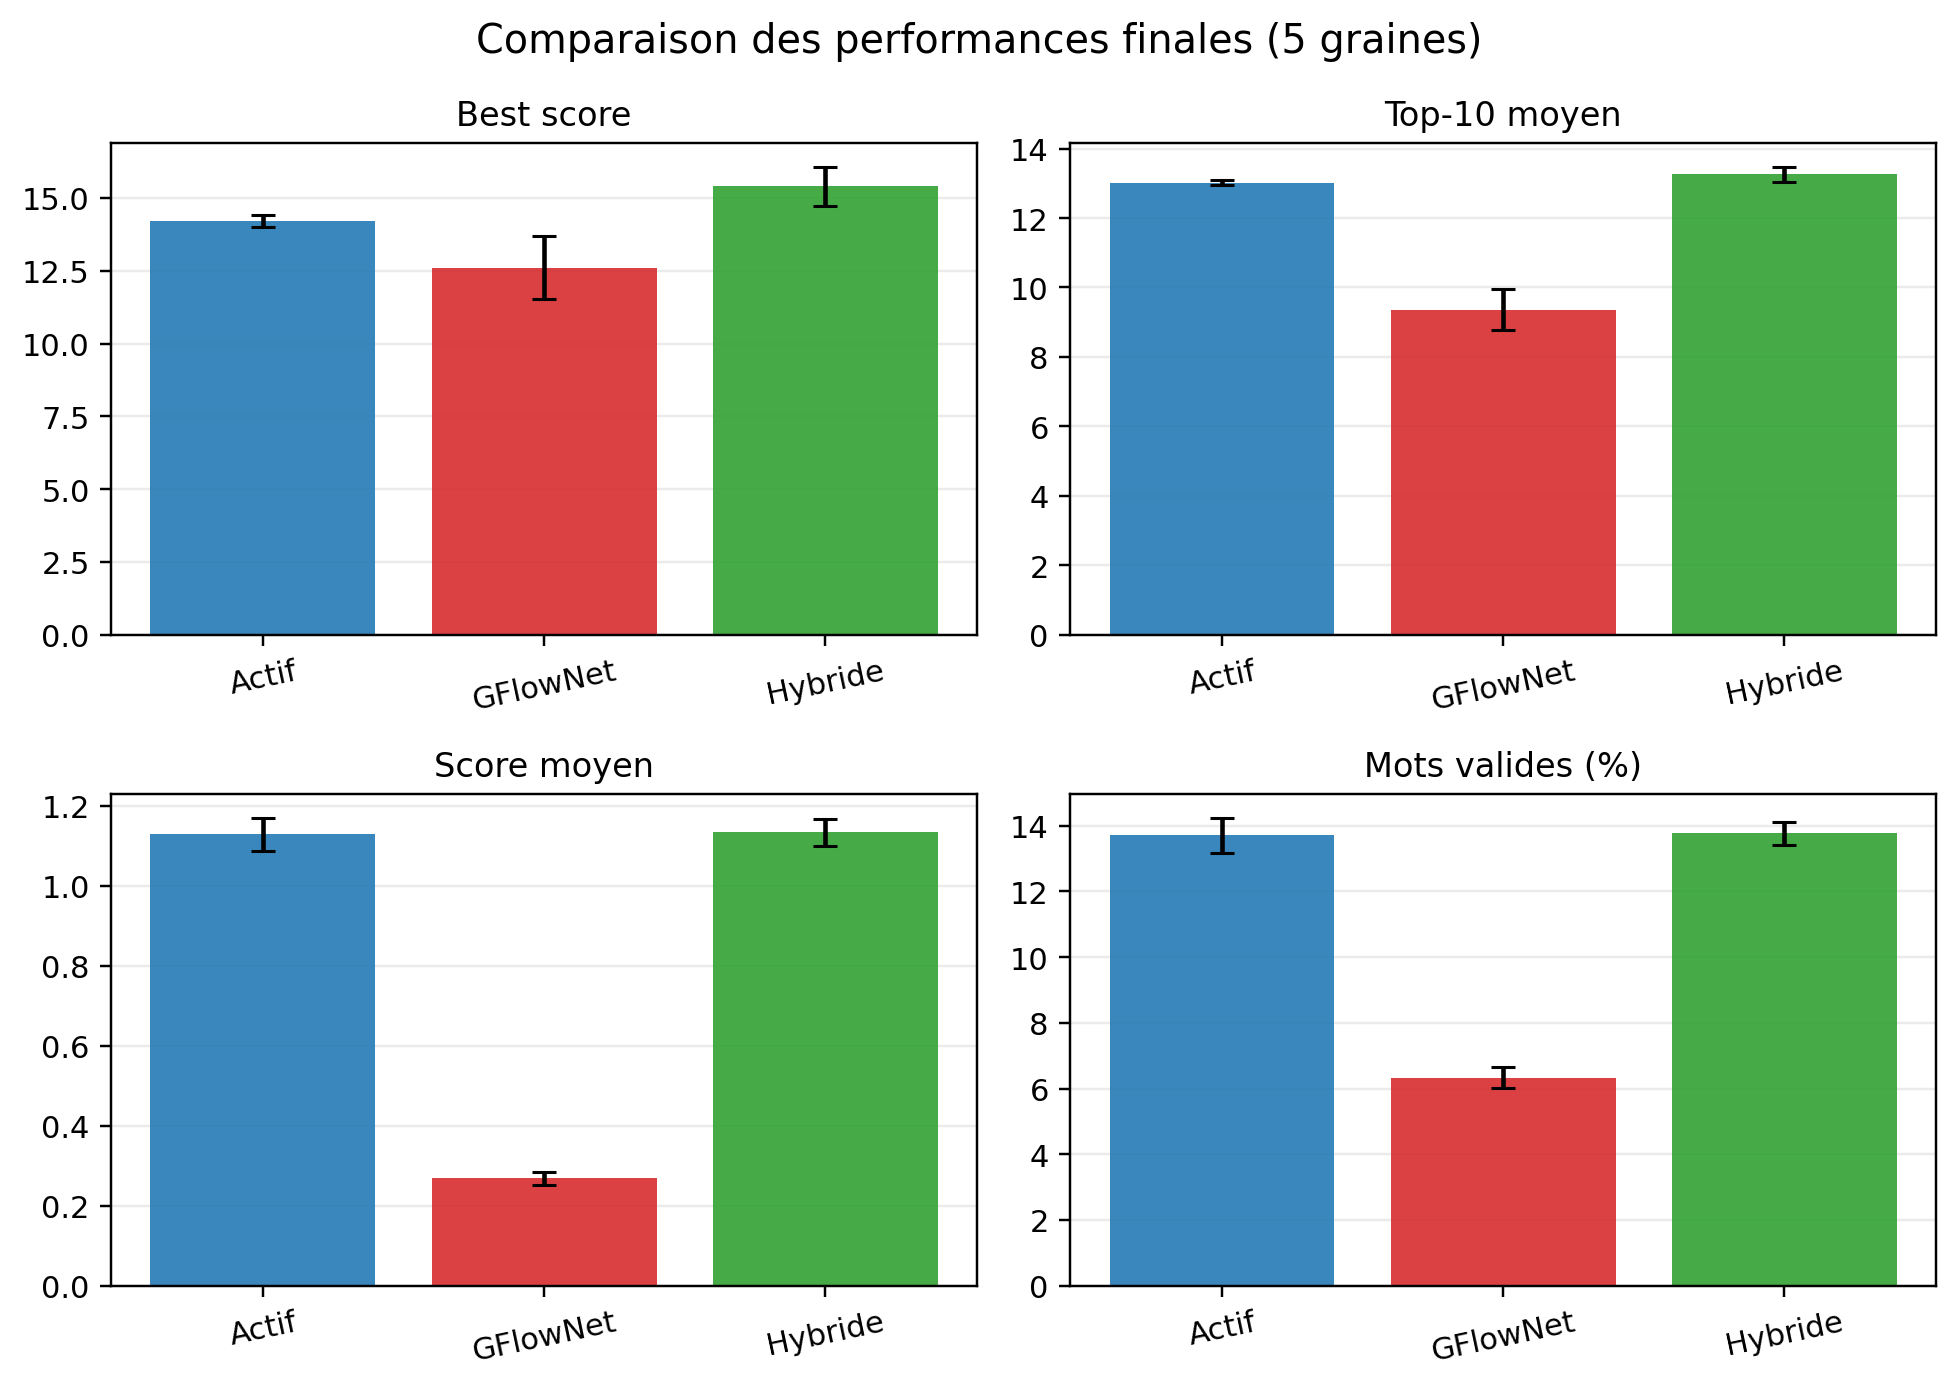
\includegraphics[width=\linewidth]{visualizations/assets/quality_overview.png}
\caption{Final-quality comparison for the tuned \(5\)-seed budget-matched sweep. These figures are generated from run \texttt{2026-03-29\_21-12-32}; the supervised baseline comes from the reference run \texttt{2026-03-29\_14-51-09}.}
\label{fig:quality}
\end{figure}

\begin{figure}[t]
\centering
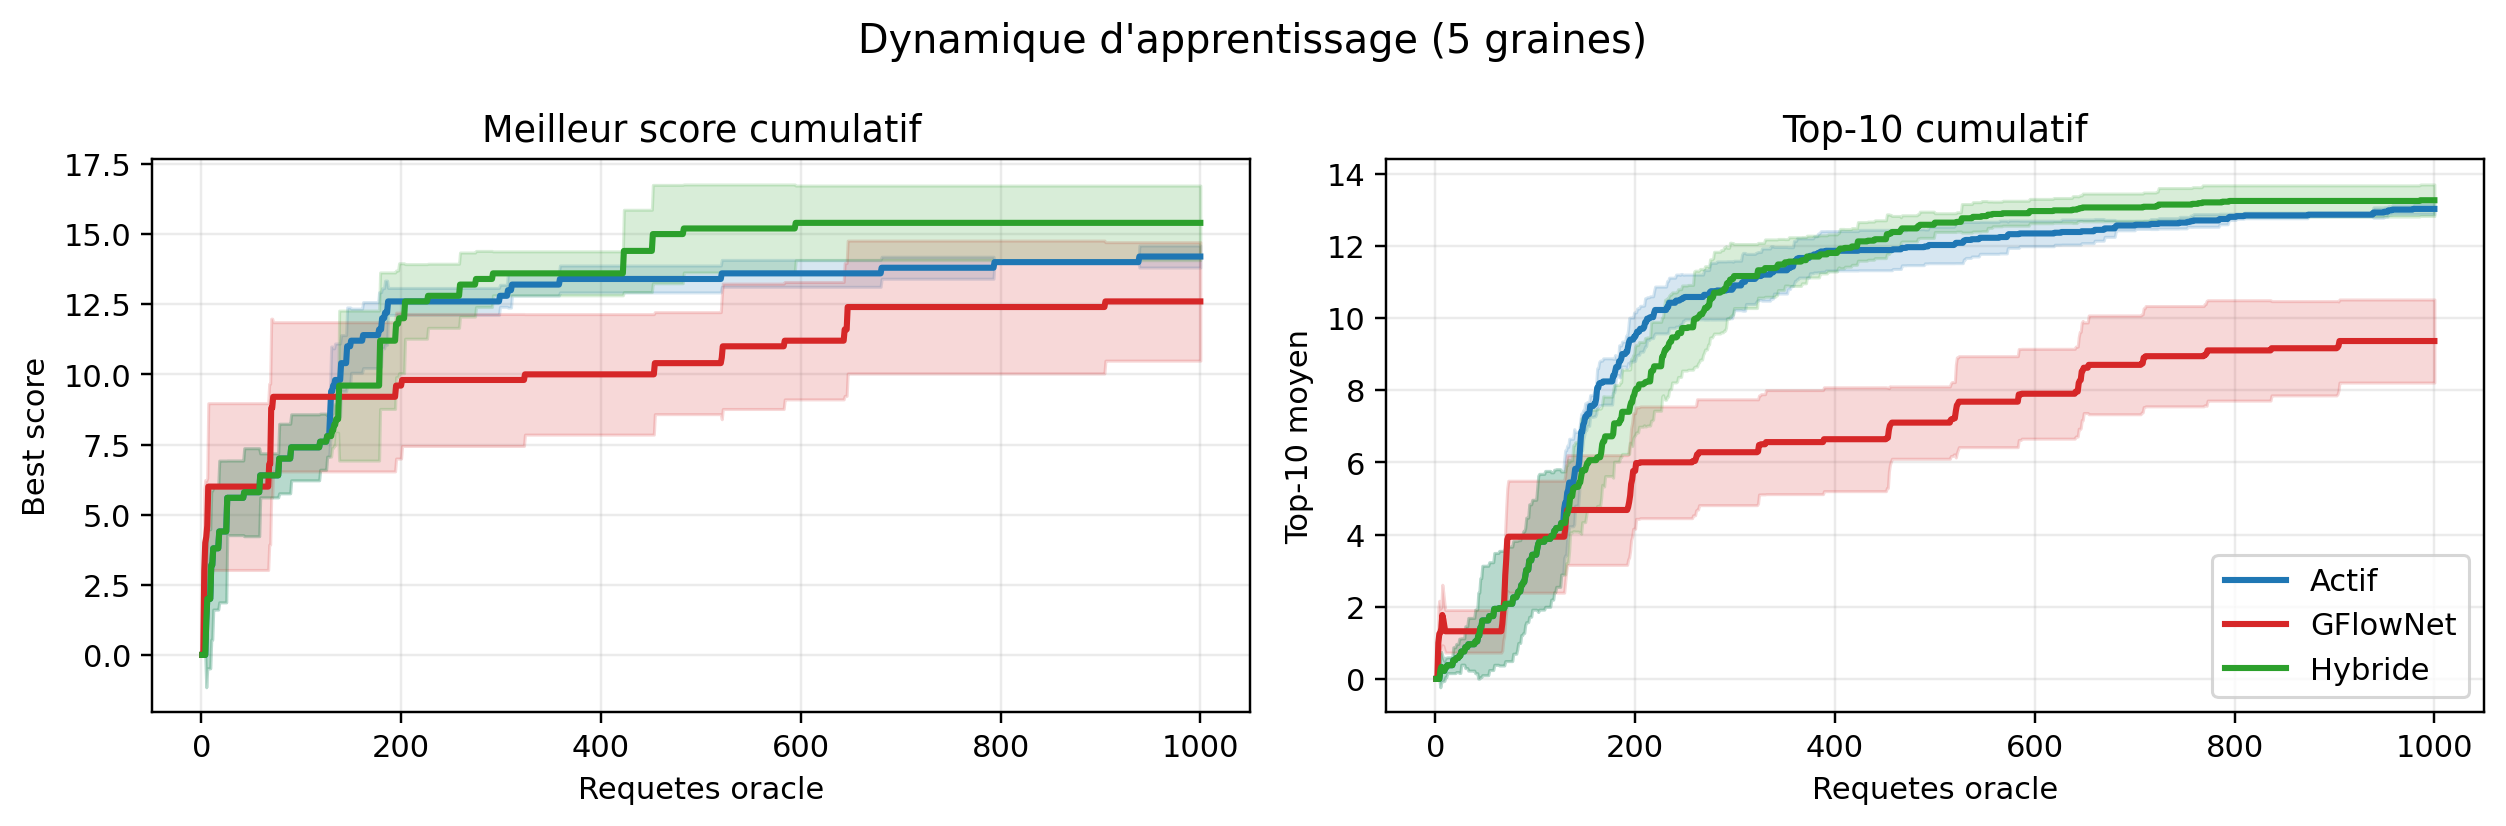
\includegraphics[width=\linewidth]{visualizations/assets/query_dynamics.png}
\caption{Learning dynamics for the tuned \(5\)-seed budget-matched sweep. The hybrid usually improves the top end of the discovered frontier, but not always the earliest query-efficiency regime.}
\label{fig:dynamics}
\end{figure}

\begin{table}[t]
\centering
\small
\caption{Tuned budget-matched comparison used for the report figures. ``Supervised'' is a reference baseline from \texttt{2026-03-29\_14-51-09}.}
\resizebox{\linewidth}{!}{
\begin{tabular}{lccccccc}
\toprule
Method & Best & Top-10 & Mean & Valid (\%) & \(Q90\) & Cheap Queries & Time (s) \\
\midrule
Supervised (ref.) & 15.67 & 12.33 & 0.793 & 10.8 & 549.7 & 8{,}191.7 & 1.45 \\
Active learning & 14.2 & 13.02 & 1.129 & 13.7 & 248.2 & 332{,}732.6 & 46.83 \\
Direct GFlowNet & 12.6 & 9.36 & 0.269 & 6.3 & 377.0 & 0.0 & 1.49 \\
Hybrid & 15.4 & 13.26 & 1.134 & 13.8 & 297.2 & 1{,}311{,}503.6 & 326.83 \\
\bottomrule
\end{tabular}
}
\label{tab:tuned}
\end{table}

This tuned comparison gives an important message: the hybrid can outperform active learning on \emph{best score} and \emph{top-10 quality}, but it does not dominate on every axis. Its \(Q90\) is worse than active learning here, and its compute cost is far higher. So the correct interpretation is not ``hybrid wins everywhere'' but rather ``hybrid can improve the quality of the discovered high-value set, at the cost of much heavier cheap computation.''

\subsection{Complete five-method run}
The most complete like-for-like archived comparison is the \(5\)-seed run \texttt{2026-03-29\_21-59-01}, which includes all five methods together.

\begin{table}[t]
\centering
\small
\caption{Complete \(5\)-seed comparison run \texttt{2026-03-29\_21-59-01}. The upper bound is not budget matched.}
\resizebox{\linewidth}{!}{
\begin{tabular}{lccccccc}
\toprule
Method & Best & Top-10 & Mean & Valid (\%) & \(Q90\) & Cheap Queries & Time (s) \\
\midrule
Supervised baseline & 15.6 & 12.08 & 0.679 & 9.4 & 517.6 & 8{,}191.6 & 2.47 \\
Active learning & 14.4 & 13.10 & 1.075 & 12.9 & 297.0 & 1{,}091{,}416.2 & 182.66 \\
Direct GFlowNet & 12.6 & 9.36 & 0.269 & 6.3 & 377.0 & 0.0 & 1.94 \\
Hybrid & 14.2 & 13.20 & 1.216 & 14.6 & 148.2 & 1{,}926{,}842.2 & 787.78 \\
Oracle-rich upper bound & 17.4 & 15.06 & 1.605 & 80.3 & 6{,}889 & 0.0 & 410.75 \\
\bottomrule
\end{tabular}
}
\label{tab:full}
\end{table}

This run makes the trade-offs clearer:
\begin{itemize}
    \item The supervised baseline is competitive on \emph{best score}, but weaker on mean score and valid-word ratio. It can get lucky, but it does not maintain as strong a frontier.
    \item Active learning is a strong budget-matched baseline. It is simpler than the hybrid and much cheaper.
    \item Direct GFlowNet is consistently the weakest budget-matched method on reward quality. Its best score, top-10 score, mean score, and valid-word ratio are all poor.
    \item The hybrid is the best method if the priority is the \emph{quality of the discovered frontier}: it is best on top-10, mean score, valid-word ratio, and \(Q90\) in this full run.
    \item The upper bound proves that GFlowNet-style search is not inherently broken; under a much looser oracle regime it reaches much stronger scores. The real issue is the mismatch between sparse rewards and a tight oracle budget.
\end{itemize}

\subsection{What is stable and what is not}
Across the two archived \(5\)-seed comparisons, the exact winner on \emph{best single score} is not perfectly stable. In the tuned sweep, the hybrid leads on best score; in the complete rerun, active learning has a slight best-score edge while the hybrid leads on frontier metrics. What \emph{is} stable is the following:
\begin{itemize}
    \item direct budget-matched GFlowNet underperforms,
    \item the hybrid is much more useful than the direct GFlowNet,
    \item active learning is a serious baseline and is hard to beat cleanly,
    \item the hybrid's gains cost substantial extra cheap computation.
\end{itemize}

\subsection{Statistical interpretation}
The repository also stores paired tests. In the complete run \texttt{2026-03-29\_21-59-01}, paired \(t\)-tests favor the hybrid over the supervised baseline on top-10 score (\(p \approx 4.67 \times 10^{-4}\)), mean score (\(p \approx 0.0038\)), and valid-word ratio (\(p \approx 0.010\)); they also favor the hybrid over active learning on mean score (\(p \approx 0.019\)) and valid-word ratio (\(p \approx 0.014\)). However, with only \(5\) seeds, the paired Wilcoxon tests remain at \(0.0625\) or above. The safest conclusion is therefore that the trends are real enough to motivate the design, but the statistical evidence is still not strong enough to claim definitive superiority in a publication-quality sense.

\section{Why the Hybrid Is Not ``Just a Full GFlowNet''}
This question is central to the project. If GFlowNets are good at sampling high-reward terminal states, why not let a full GFlowNet handle the hybrid search end-to-end?

The answer is that the hybrid problem is \emph{not only} a reward maximization problem. It is also a \emph{budget allocation} problem. A full GFlowNet is naturally trained to sample states proportional to some reward signal, but in our setting the expensive decision is: \emph{which candidates deserve a real oracle query right now?} That decision depends on more than predicted reward.

There are four concrete reasons we did not collapse the hybrid into a full end-to-end GFlowNet:
\begin{enumerate}
    \item \textbf{Real oracle queries are the scarce resource.} The GFlowNet is excellent as a cheap proposal engine, but the expensive part is deciding which proposals are worth spending real budget on. Active-learning acquisition functions are explicitly designed for that purpose.
    \item \textbf{The surrogate is non-stationary.} In the hybrid loop, the surrogate changes after every round of new real labels. A full GFlowNet trained on that moving target would need frequent retraining or continual adaptation, which is expensive and unstable.
    \item \textbf{Reward alone is not enough.} Real-query selection should depend on uncertainty, diversity, and sometimes exploitation pressure. A plain surrogate-reward GFlowNet samples high predicted reward states; it does not directly optimize information gain or batch diversity.
    \item \textbf{The project already observed the failure mode empirically.} An early hybrid prototype that effectively used ``more GFlowNet, earlier, and more often'' spent enormous fake-oracle compute for mediocre returns.
\end{enumerate}

So the final design uses the GFlowNet where it is strongest: \emph{sampling structured, high-potential candidates from a cheap proxy reward}. It does \emph{not} ask the GFlowNet to replace uncertainty-aware, diversity-aware real-oracle selection.

\section{What We Tried That Did Not Work Well}
\subsection{Direct oracle-access GFlowNet under tight budget}
The cleanest negative result in the repository is the direct GFlowNet itself. In both archived \(5\)-seed comparisons, it is clearly worse than active learning and the hybrid. In the complete run, its mean best score is \(12.6\), its top-10 mean is only \(9.36\), and only \(6.3\%\) of its queried states are valid words. This is the strongest evidence that sparse rewards plus a small real-oracle budget are a bad regime for a pure reward-driven GFlowNet.

\subsection{An early always-on hybrid prototype}
The file \texttt{hybrid\_multi\_seed.log} and the archived single-seed run \texttt{2026-03-27\_11-45-12\_seed0} preserve an earlier hybrid design that started using the surrogate-backed GFlowNet immediately and refreshed it aggressively. That run ended with:
\begin{itemize}
    \item best score \(11.0\),
    \item top-10 score \(9.1\),
    \item \(Q90 = 638\),
    \item \(3{,}584{,}000\) fake-oracle queries,
    \item \(3{,}805{,}382\) cheap-model queries,
    \item runtime of about \(2513.5\) seconds.
\end{itemize}

This was a decisive negative result. It showed that simply training the GFlowNet from round \(0\) and retraining it frequently does \emph{not} automatically improve search. Instead, it can waste huge compute budgets while the surrogate is still too weak to give the GFlowNet a meaningful landscape.

The final hybrid design is a direct response to this failure:
\begin{itemize}
    \item wait before turning on the GFlowNet,
    \item require a minimum number of positive examples,
    \item retrain less frequently,
    \item warm-start instead of starting from scratch,
    \item keep random, mutation, and local-search proposals in the pool.
\end{itemize}

\subsection{Naive exploration without linguistic structure}
The code comments around the plausibility bonus and the final default configs strongly suggest another lesson learned during development: purely uncertainty-driven search in this domain tends to chase strange, low-density, non-word strings. In other words, raw uncertainty is easy to maximize on nonsense sequences, but nonsense sequences usually return reward \(0\). This is why the final codebase consistently uses:
\begin{itemize}
    \item vocabulary-aware \emph{n}-gram sampling,
    \item word-likeness bonuses in acquisition,
    \item domain features inside the surrogate.
\end{itemize}
Even when these tricks do not solve the optimization problem alone, they break the worst failure mode: repeatedly spending budget on obviously implausible candidates.

\section{Limitations}
The current project is successful as an engineering and experimental study, but several limitations remain:
\begin{itemize}
    \item only \(5\) seeds are used in the main comparisons,
    \item the latest figure sweep and the latest complete five-method run are not the exact same run,
    \item the upper bound is not budget matched and should not be read as a fair competitor,
    \item the hybrid still has high computational cost,
    \item all budget-matched methods remain very far from the configured optimum score of \(45\).
\end{itemize}

Another subtle limitation is metric interpretation. For example, direct GFlowNet has very high mode coverage, but the covered modes are often mediocre. So diversity metrics alone are not sufficient; they must be read together with reward quality.

\section{What Should Be Improved Next}
The most important future work follows directly from the results:

\subsection{1. Improve surrogate quality and calibration}
The entire hybrid depends on the surrogate. If the surrogate is wrong, the fake-oracle GFlowNet is wrong too. Better calibrated uncertainty and stronger ranking quality should be the first priority, because both active learning and the hybrid are bottlenecked by surrogate quality.

\subsection{2. Make the hybrid cheaper}
The hybrid's biggest practical weakness is compute cost. The next step should be to reduce fake-oracle and cheap-model queries through lighter refresh schedules, more selective GFlowNet retraining, or incremental updates rather than repeated near-full retraining.

\subsection{3. Strengthen the final exploitation phase}
The hybrid often improves the \emph{frontier}, but not always the single best sample. That suggests a missing endgame. A stronger final exploitation stage, such as a sharper local search around top hybrid proposals or a final exploitation-focused rescorer, could improve best-score performance without discarding the frontier advantage.

\subsection{4. Explore acquisition-aware GFlowNet objectives}
The natural research extension is not ``replace the hybrid with a full GFlowNet,'' but rather make the surrogate-backed GFlowNet better aligned with active-learning utility. For example, a future proxy could combine predicted reward, uncertainty, and diversity more directly, instead of using the GFlowNet only on surrogate reward and then letting acquisition repair the mismatch afterward.

\subsection{5. Run broader ablations and more seeds}
The repository already contains ablation runners, but the main report still needs more extensive ablation evidence and more seeds for stronger nonparametric significance. This is essential before making strong scientific claims.

\subsection{6. Improve validity modeling}
Even the stronger budget-matched methods still query many invalid words. The valid-word ratio of the hybrid in the complete run is only \(14.6\%\), far below the oracle-rich upper bound's \(80.3\%\). Better dictionary-conditioned generation or better validity prediction could convert much more of the fixed oracle budget into useful labels.

\section{Conclusion}
The project achieved its main goal: it built and compared a full stack of methods for budgeted Scrabble exploration, and it identified clearly where GFlowNets help and where they do not. The strongest negative result is that a direct oracle-access GFlowNet is not competitive under a tight real-query budget. The strongest positive result is that a GFlowNet \emph{can} still be useful when it is embedded inside a broader active-learning loop and used as a structured proposal mechanism rather than as the entire decision-maker.

So the final takeaway is precise. We did not avoid a ``full GFlowNet hybrid'' because GFlowNets are bad; we avoided it because the hybrid problem is fundamentally about \emph{budget-aware selection under uncertainty}, not just reward-proportional sampling. In this project, the best use of the GFlowNet was to help generate promising candidates cheaply, while the active-learning machinery remained responsible for deciding where the scarce real oracle budget should go.

\end{document}
